% Summary diagram (Section 5 of ARCHITECTURE.md) — compile standalone with:
%   pdflatex diagram.tex
\documentclass[border=6pt]{standalone}
\usepackage{tikz}
\usetikzlibrary{arrows.meta, positioning, fit}

\begin{document}
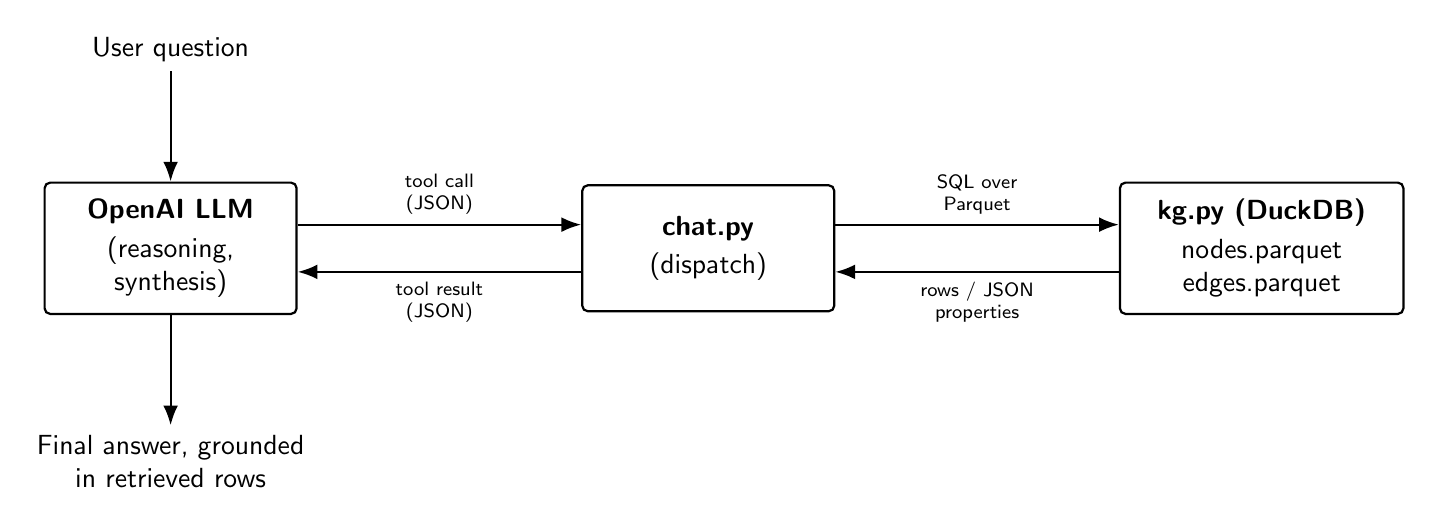
\begin{tikzpicture}[
    font=\sffamily,
    box/.style={
        draw, thick, rounded corners=2pt,
        minimum width=3.2cm, minimum height=1.6cm,
        align=center, inner sep=6pt
    },
    lbl/.style={font=\sffamily\scriptsize, align=center, text width=3.4cm},
    arrow/.style={-{Latex[length=2.5mm]}, thick}
]

% -- top: user question --
\node[align=center] (question) {User question};

% -- main pipeline boxes --
\node[box, below=1.4cm of question] (llm)
    {\textbf{OpenAI LLM}\\[2pt] (reasoning,\\ synthesis)};

\node[box, right=3.6cm of llm] (chatpy)
    {\textbf{chat.py}\\[2pt] (dispatch)};

\node[box, right=3.6cm of chatpy, minimum width=3.6cm] (kgpy)
    {\textbf{kg.py (DuckDB)}\\[2pt] nodes.parquet\\ edges.parquet};

% -- bottom: final answer --
\node[align=center, below=1.4cm of llm] (answer)
    {Final answer, grounded\\ in retrieved rows};

% -- vertical arrows --
\draw[arrow] (question) -- (llm);
\draw[arrow] (llm) -- (answer);

% -- llm <-> chat.py --
\draw[arrow] ([yshift=3mm]llm.east) -- node[lbl, above]{tool call\\(JSON)} ([yshift=3mm]chatpy.west);
\draw[arrow] ([yshift=-3mm]chatpy.west) -- node[lbl, below]{tool result\\(JSON)} ([yshift=-3mm]llm.east);

% -- chat.py <-> kg.py --
\draw[arrow] ([yshift=3mm]chatpy.east) -- node[lbl, above]{SQL over\\Parquet} ([yshift=3mm]kgpy.west);
\draw[arrow] ([yshift=-3mm]kgpy.west) -- node[lbl, below]{rows / JSON\\properties} ([yshift=-3mm]chatpy.east);

\end{tikzpicture}
\end{document}
